\documentclass[border=10pt]{standalone}

\usepackage{tikz}
\usepackage{tikzsymbols}
\usetikzlibrary{calc,patterns,shapes.geometric}

\def\centerarc[#1](#2)(#3:#4:#5){\draw[#1] ($(#2)+({#5*cos(#3)},{#5*sin(#3)})$) arc (#3:#4:#5);}

\begin{document}
	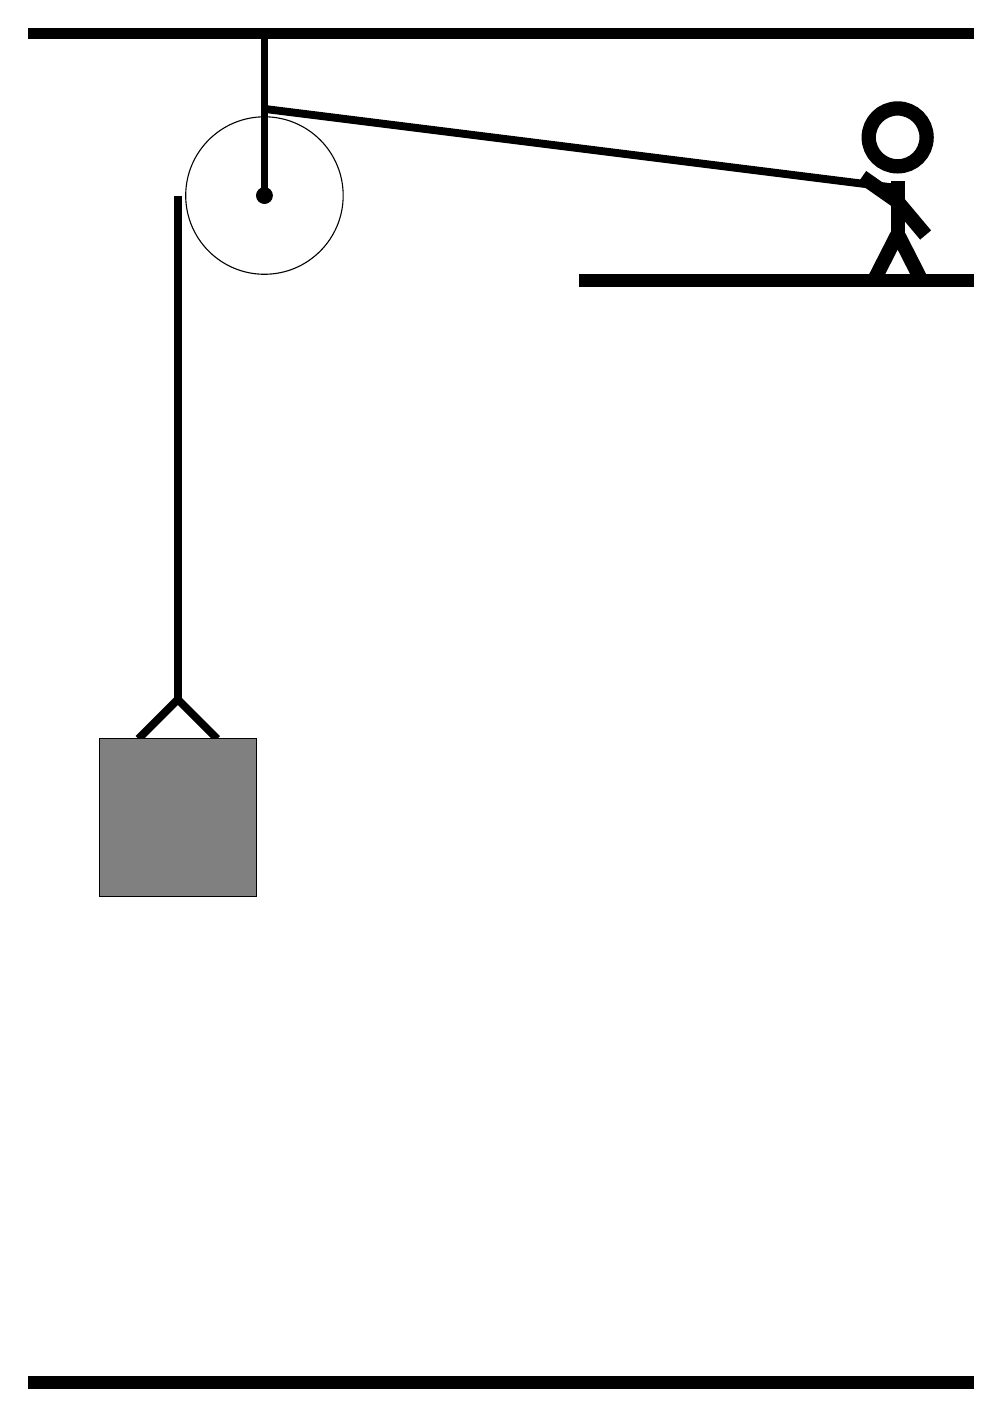
\begin{tikzpicture}
		%%%%% START %%%%%
		\draw[fill=black] (-2, 14) rectangle (10, 14.125);
		
		\draw (1, 12) circle (1);
		\draw[fill=black] (1, 12) circle (0.1);
		\draw[line width=1mm] (1, 14) -- (1, 12);
		
		\draw[line width=1mm](-0.6, 5.1) --  (-0.1, 5.6) -- (0.4, 5.1);
		\draw[fill=black!50] (-1.1, 5.1) rectangle (0.9, 3.1);
		
		\draw[line width=1mm](-0.1, 12) -- (-0.1, 5.6);
		\centerarc[line width=1mm](1, 12)(90:180:1.1)
		\draw[line width=1mm](1, 13.1) -- (9, 12.1);
		
		\node at (9, 12) {\Strichmaxerl[10][-35][-50]};
		\draw[fill=black] (5, 11) rectangle (10, 10.85);
		
		\draw[fill=black] (-2, -3) rectangle (10, -3.15);
		%%%%% END %%%%%
	\end{tikzpicture}
\end{document}